\clearpage{\pagestyle{empty}\cleardoublepage}
\chapter{Block RAM}


Nel nostro progetto descritto in precedenza, per semplicit\`a  abbiamo considerato l'ipotesi di avere tempi d'accesso nulli alla cache e alla memoria principale. Ovviamente ci\`o non accadrebbe in un progetto reale che preveda l'utilizzo di cache al fine di velocizzare l'accesso ai dai evitando in caso di HIT l'accesso alla memoria RAM. Per curiosit\`a e completezza nell'affrontare le tematiche relative al nostro progetto, abbiamo voluto approfondire le problematiche riguardanti le temporizzazioni per gli accessi in memoria che un progetto reale impone. Per far ci\`o abbiamo considerato i dispositivi di memoria che una FPGA d\`a a disposizione ad un progettista per implementare una memoria RAM e gestirne gli accessi in lettura e scrittura.\\

Nel nostro caso abbiamo analizzato le caratteristiche dell'FPGA della famiglia Spartan-3 di Xilinx \cite{xil1}, che per gestire la memorizzazione di dati consente due possibili soluzioni:
\begin{enumerate}
\item  Memorie RAM distribuite sulla scheda, di piccole dimensioni e rapidissimo accesso, utilizzate tipicamente come registri temporanei d'appoggio.
\item Le Block RAM, ovvero blocchi di memoria RAM statica con tempi d'accesso non nulli e un' ampia capacit\`a potenziale di memorizzazione, in relazione alle caratteristiche tecniche della scheda FPGA utilizzata. 
\end{enumerate}

\section{Caratteristiche e segnali della Block Ram}

La memoria RAM presente su una FPGA Spartan-3 \cite{xil2} viene implementata tramite una serie di Block RAM ripartite in colonne il cui numero e capacit\`a dipende dalle caratteristiche stesse della scheda utilizzata. Dal punto di vista implementativo le Block RAM sono realizzate tramite 18,432 celle di memoria SRAM che consentono pertanto di memorizzare 18 Kbits di cui 16 Kbits di dato e 2 Kbits utilizzati tipicamente per memorizzare i bit di parit\`a relativi ai dati memorizzati o in alternativa come spazio di memorizzazione aggiuntivo.\\

L'accesso alla Block RAM pu\`o avvenire o in modalit\`a Single-Port utilizzando una sola porta dati (A o B) oppure in Dual-Port  tramite 2 porte indipendenti A e B che consentono di effettuare operazioni di lettura e scrittura sull'intero spazio di memoria del dispositivo (anche con sovrapposizioni).

\begin{figure}[!h]
\centering
% 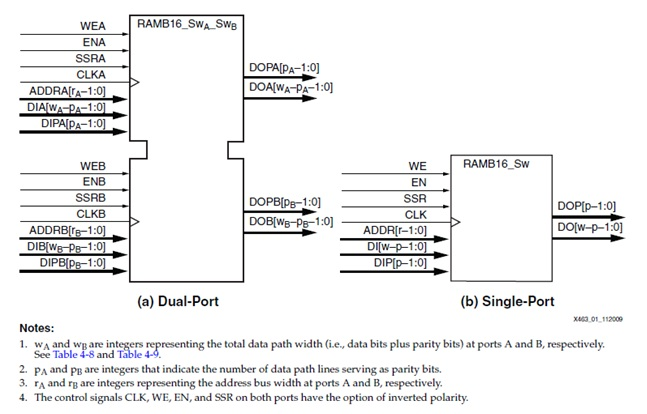
\includegraphics[scale=0.8]{img/blockRam/pinoutPorte.jpg}
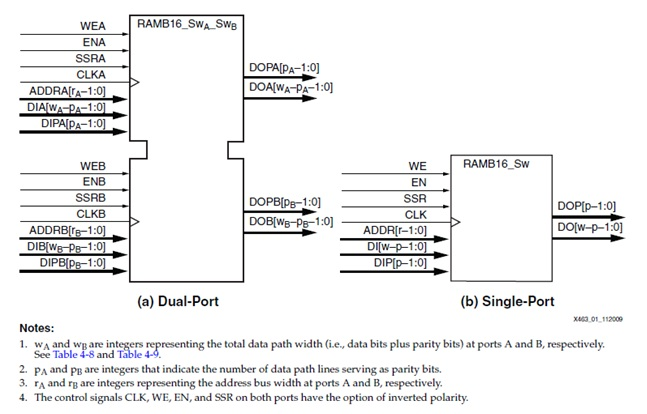
\includegraphics[width=\textwidth]{img/blockRam/pinoutPorte.jpg}
\caption{Block Ram Single-Port e Dual-Port}
\label{fig:operaz}
\end{figure}


Ogni porta della Block RAM si interfaccia con due bus dati (distinti per l'input e per l'output), con il bus degli indirizzi e dispone di una serie di segnali di comando atti ad abilitare il dispositivo e a gestire operazioni di lettura o scrittura. La tabella in Fig.\ref{fig:segnaliBlockRam} racchiude i principali segnali in input e output sulla Block Ram sia in Single-Port che in Dual-Port.

\begin{figure}[!h]
\centering
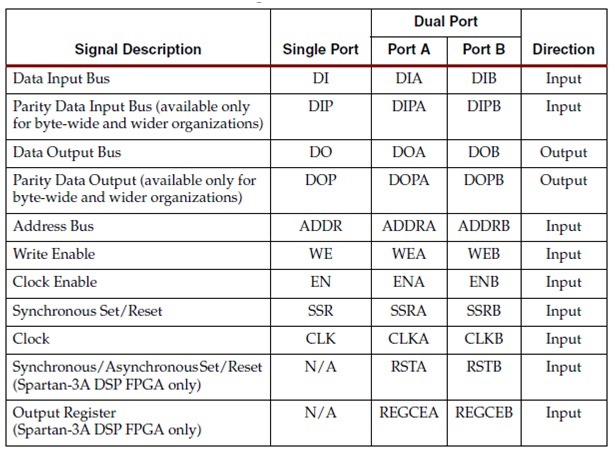
\includegraphics[width=\textwidth]{img/blockRam/segnali.jpg}
\caption{Segnali della Block Ram Single-Port e Dual-Port}
\label{fig:segnaliBlockRam}
\end{figure}

Segnali di comando in Single-Port:

\begin{itemize}
  \item \texttt{EN}: Enable consente di abilitare il dispositivo e qualora non siano asseriti WE (write enable) o SSR (syncronous set/reset), il segnale comanda la lettura del dato all'indirizzo specificato sul bus degli indirizzi ADDR sul fronte positivo del clock;
  \item \texttt{WE}: Write Enable consente di comandare un ciclo di scrittura in memoria all'indirizzo specificato sul bus degli indirizzi ADDR (con EN asserito). La peculiarit\`a delle operazioni di scrittura \`e che sono sempre precedute o seguite da una lettura del dato al medesimo indirizzo sulla base del comportamento configurabile tramite l'attributo \texttt{WRITE\_MODE} che analizzeremo in seguito; 
  \item \texttt{SSR}: Syncronous Set/Reset consente di assegnare '1' o non '0' i latch di ouput sul bus dati in accordo col valore dell'attributo \texttt{SRVAL} specificato in fase di inizializzazione (X"00000" a default);
  \item \texttt{REGCE}: Output Register Enable consente in fase di  lettura da ram di salvare il dato letto in un output register;
  \item \texttt{CLK}:  \`e il clock e si pu\`o configurare se la memoria debba essere sensibile ai fronti di salita o di discesa:
\item \texttt{GSR}: Global Set/Reset segnale di sistema utilizzato in fase di inizializzazione del sistema per inizializzare la Block RAM (non disponibile all'esterno su un pin).
\end{itemize}

C'\'e inoltre la possibilit\`a di configurare le polarit\`a di ogni segnale di comando se da considerarsi asserito alto o basso.\\

Interfacciamento ai bus:\\

\begin{itemize}
  \item \texttt{ADDR}: bus degli indirizzi la cui larghezza [NA:0] dipende dalla configurazione della Block RAM;
  \item \texttt{DI}: Data Input Bus [ND:0] (l'ampiezza del dato da trasferire dipende dalla configurazione della Block RAM);
  \item \texttt{DO}: Data Output Bus;
  \item \texttt{DIP}: Data Input Parity Bus (nei bit pi\`u significative del Bus Dati di Input);
  \item \texttt{DOP}: Data Output Parity Bus (nei bit pi\`u significative del Bus Dati di Output);
\end{itemize}

Possibili configurazioni e organizzazioni della Block RAM sono illustrate in Fig. \ref{fig:ram_org}.\\

\begin{figure}[!h]
\centering
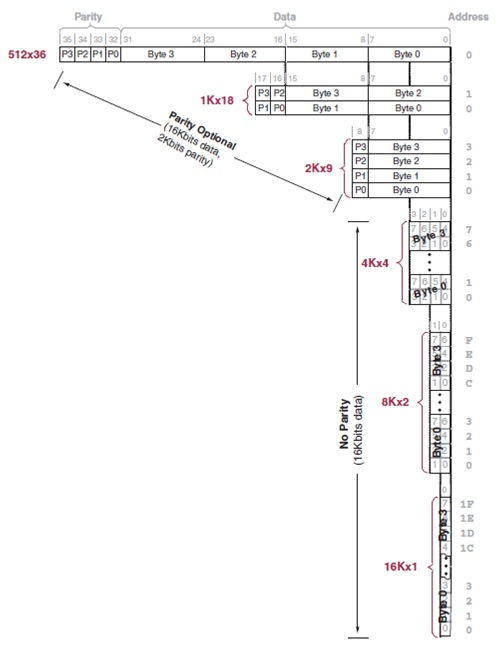
\includegraphics[width=\textwidth]{img/blockRam/organInterna.jpg}
\caption{Possibili organizzazioni interne della Block Ram}
\label{fig:ram_org}
\end{figure}

Ad esempio, se si volesse utilizzare la Block Ram come memoria Ram per un processore DLX, la configurazione necessaria sarebbe la 512x36. Tale configurazione d\'a la possibilit\'a di accedere al dispositivo fino a 36 bit contemporaneamente, di cui 32 bit di dato e 4 bit di parit\`a. Con tale configurazione la Block Ram (di 18 Kbit) conterrebbe 512 entry (memory-depth) da 36 bit (infatti 512x36 bit = 18 Kbit).

\section{Configurazione della Block RAM}

La configurazione della Block RAM avviene tramite una serie di attributi nella sezione \texttt{generic (...)} dei componenti RAM disponibili nelle librerie di sistema tramite i quali si pu\`o settare in base alle specifiche di progetto l'organizzazione interna, la dimensione e diverse altre caratteristiche della Block Ram come il comportamento WRITE\_MODE in scrittura.\\
Generalmente il numero di porte della RAM e la sua organizzazione interna possono essere specificati utilizzando Xilinx Core Generator che consente di configurare tramite un wizard la Block Ram ottenendo direttamente il codice VHDL del componente ram desiderato oppure si possono utilizzare i tipi VHDL  gi\`a associati alla Block Ram RAMB16\_Sn dove n corrisponde all'ampiezza del dato + parit\`a (Fig.\ref{fig:tipi_br}).

\begin{figure}[!h]
\centering
%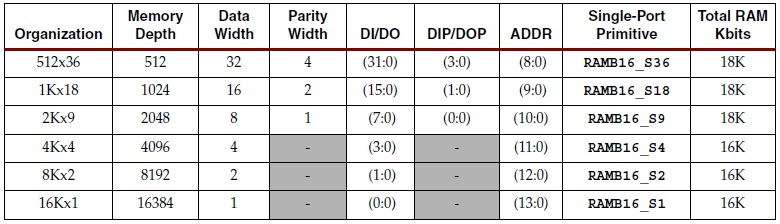
\includegraphics[width=\textwidth]{img/blockRam/tabTipiRam.jpg}
 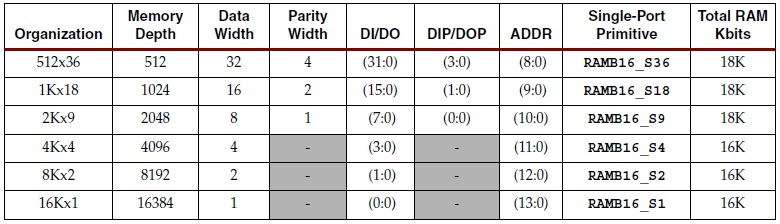
\includegraphics[width=\textwidth]{img/blockRam/tabTipiRam.jpg}
\caption{La tabella mostra le diverse tipologie di RAMB\_Sn ottenibili dalla Block Ram in base all'organizzazione interna desiderata}
\label{fig:tipi_br}
\end{figure}

\subsection{Inizializzazione del contenuto e attributi di configurazione}
\begin{itemize}
  \item \texttt{INIT\_xx - INITP\_xx}
A default la Block Ram \`e inizializzata a tutti 0, ma \`e possibile inizializzarne il contenuto in diversi modi o direttamente tramite Core Generator al momento della configurazione del componente oppure tramite opportuni attributi VHDL come INIT\_xx e INITP\_xx.\\ 
Nel primo caso si passa direttamente un file di coefficienti (.coe) che definisce in primo luogo la base numerica dei dati da inserire e in seguito l'elenco dei dati elencati a partire dalla parte bassa della memoria fino agli indirizzi alti. Un esempio della struttura di tale file \`e il seguente:\\

\texttt{memory\_inizialization\_radix=16;\\
	memory\_inizialization\_vector=80, 0F, 00, ..., 82;\\}

In alternativa si utilizzano direttamente 64 attributi VHDL \texttt{INIT\_xx} (da \texttt{INIT\_00} a \texttt{INIT\_3F} in Fig.\ref{fig:attrInit_br}) che consentono di inizializzare le 64 zone da 256 bit con cui \`e ripartita la memoria. Gli indirizzi del blocco di memoria da inizializzare identificati da \texttt{xx} sono calcolabili nel seguente modo dopo aver convertito l'indirizzo esadecimale xx nel corrispondente indirizzo decimale yy:\\

indirizzo iniziale del blocco xx = [(yy + 1) * 256] - 1\\
indirizzo finale del blocco xx = yy * 256\\

\begin{figure}[!h]
\centering
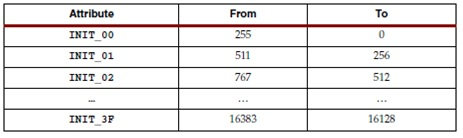
\includegraphics[scale=0.8]{img/blockRam/init.jpg}
\caption{Attributi di Inizializzazione del contenuto della Block Ram}
\label{fig:attrInit_br}
\end{figure}

INITP\_xx sono attributi analoghi che consentono di inizializzare i bit di parit\`a presenti in memoria (da INITP\_00 a INITP\_07).
\item \texttt{INIT}  \`e l'attributo utilizzato in fase di inizializzazione per settare il valore iniziale del registro di output quando viene asserito il segnale GSR.\\

\item \texttt{WRITE\_MODE}  \`e l'attributo che consente di specificare il comportamento della Block Ram e dei latch di output durante un ciclo di scrittura. I possibili valori sono i seguenti:

\begin{enumerate}
\item \texttt{WRITE\_FIRST} \`e  il valore di default e comporta un comportamento Read after Write della memoria, ovvero durante un ciclo di scrittura il dato in input viene contemporaneamente scritto alla locazione di memoria indicata dall'indirizzo e memorizzato e reso disponibile sui latch di output.\\
Nel caso di utilizzo in Dual-Port si ha l'effetto collaterale di un'invalidazione del contenuto del registro di output dell'altra porta, causando pertanto potenziali problemi di conflitto in caso di scrittura e lettura contemporanei sulle due porte.(Fig.\ref{fig:write_first}).

\begin{figure}
\centering
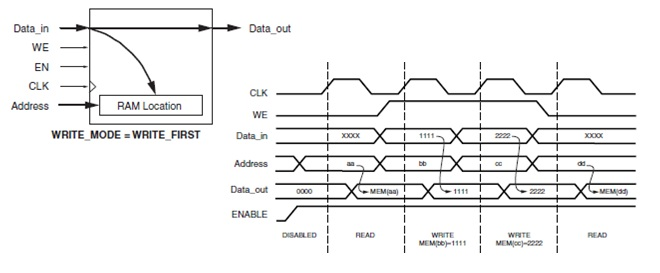
\includegraphics[width=\textwidth]{img/blockRam/writeFirst.jpg}
\caption{WRITE\_MODE = WRITE\_FIRST}
\label{fig:write_first}
\end{figure}

\item \texttt{READ\_FIRST} determina un comportamento Read before Write, ovvero prima si carica nei latch di output il dato presente alla locazione di memoria specificata dall'indirizzo e poi lo si sovrascritto in memoria con l'operazione di scrittura. Le temporizzazioni e il comportamento dettagliato in tale modalit\`a sono illustrati in Fig.\ref{fig:read_first}. 

\begin{figure}
\centering
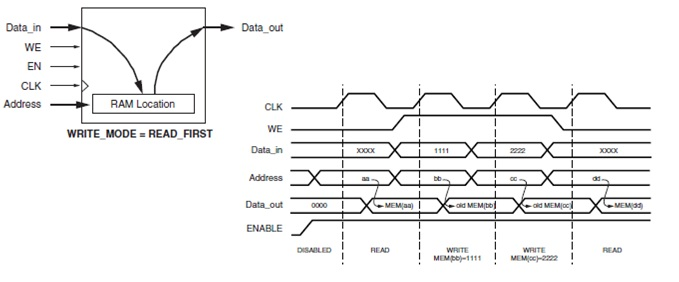
\includegraphics[width=\textwidth]{img/blockRam/readFirst.jpg}
\caption{WRITE\_MODE = READ\_FIRST}
\label{fig:read_first}
\end{figure}

\item \texttt{NO\_CHANGE} determina un comportamento classico di scrittura in memoria senza alcun aggiornamento del dato contenuto nel registro in output (temporizzazioni e funzionamento in Fig.\ref{fig:no_change}). Nel caso di utilizzo in Dual-Port si ha come side-effect l'invalidazione del contenuto del registro di output dell'altra porta. %\\\\
\end{enumerate}

\begin{figure}
\centering
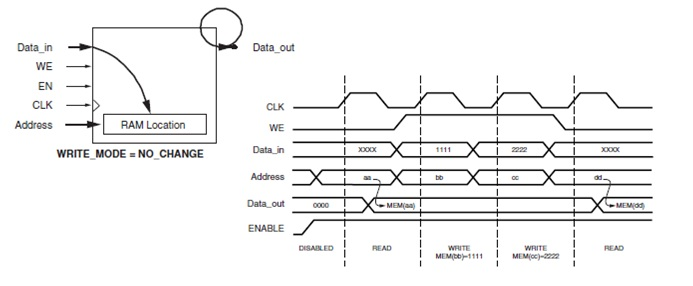
\includegraphics[width=\textwidth]{img/blockRam/noChange.jpg}
\caption{WRITE\_MODE = NO\_CHANGE}
\label{fig:no_change}
\end{figure}

\end{itemize}

\section{Operazioni della Block RAM}

Di seguito viene riportato l'elenco delle operazioni che la Block Ram  \`e in grado di gestire e dei relativi segnali impiegati:

\begin{itemize}
  \item \textbf{Global Set/Reset}: segue la fase di inizializzazione iniziale del contenuto della Block Ram in cui si inizializza la ram o a tutti zeri (default) o ai valori impostati con gli attributi \texttt{INIT\_xx}. Tale segnale serve per inizializzare lo stato dei flipflop e registri di output che vengono settati in base al valore specificato dall'attributo \texttt{INIT} (0 a default). 

\item \textbf{RAM Disabled}: se il segnale \texttt{EN} non  \`e asserito la ram mantiene il proprio stato. Ogni operazione prevede che EN venga asserito affinch\`e la RAM sia attiva.

\item \textbf{Synchronous Set/Reset}: \`e l'operazione conseguente all'asserzione contemporanea dei segnali \texttt{EN} e \texttt{SSR}. Tale operazione comporta la re inizializzazione dei registri di output al valore specificato dall'attributo\texttt{ SRVAL}.

\item \texttt{WE} + \texttt{SSR} comporta un ciclo di scrittura in cui il dato in input viene salvato in memoria all'indirizzo presente sul bus degli indirizzi, mentre nei latch di output viene impostato il valore dell'attributo SRVAL.

\item \textbf{READ}: la lettura sulla Block RAM avviene in modo sincrono, quindi sul fronte positivo del clock qualora sia asserito il solo segnale di \texttt{EN}.

\item \textbf{WRITE}: la scrittura sulla Block RAM avviene in modo sincrono sul fronte positivo del clock e qualora siano asseriti contemporaneamente \texttt{EN} + \texttt{WE}. La scrittura del dato in input sui pin dell'Input Data Bus avviene all'indirizzo specificato e tale operazione  \`e affiancata contemporaneamente dalla lettura del dato alla stessa locazione di memoria che viene reso disponibile in lettura e caricato sui latch di output. Naturalmente la politica con la quale avviene tale operazione di scrittura e lettura simultanea  \`e definita dal valore dell'attributo \texttt{WRITE\_MODE}.
\end{itemize}

La tabella mostrata in Fig.\ref{fig:operazioniBlockRam} racchiude quanto detto in precedenza e associa ad ogni operazione i valori dei segnali associati.

\begin{figure}[!h]
\centering
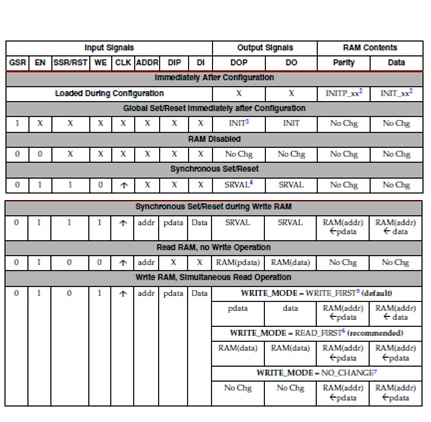
\includegraphics{img/blockRam/operazioni.jpg}
\caption{Tabella delle operazioni ed dei segnali utilizzati sulla Block Ram}
\label{fig:operazioniBlockRam}
\end{figure}

\section{Conflitti d'accesso in Block RAM Dual-Port}
Utilizzando la Block RAM in modalit\`a Dual-Port  si ha la possibilit\`a di utilizzare contemporaneamente le due porte per accedere alla memoria sia in lettura e scrittura. Mentre da un lato ci\`o consente di aumentare lo throughput complessivo dei dati trasferiti, dall'altro vi sono potenziali problemi di conflitto negli accessi simultanei alle stesse celle di memoria.\\

Le condizioni di potenziale conflitto sono le seguenti:

\begin{enumerate}
	\item Scrittura simultanea sulle due porte alla stessa locazione di memoria.\\
	Tale situazione non ha un meccanismo di arbitraggio per far fronte ad accessi in scrittura simultanei, ma l'effetto prodotto \`e quello di comportare l'invalidazione del contenuto dell'area di memoria coinvolta.
	\item Conflitti per temporizzazioni clock-to-clock tra le due porte.\\
Ci\`o accade a causa dei clock diversi che comandano le operazioni tra le due porte che sono troppo ravvicinati tra loro e il clock della porta in lettura non rispetta i tempi di setup per l'accesso in scrittura al dispositivo (arriva troppo presto quando ancora la scrittura in memoria non ha terminato). Un esempio \`e illustrato in Fig.\ref{fig:conflittiTemp}.\\

\begin{figure}[!h]
\centering
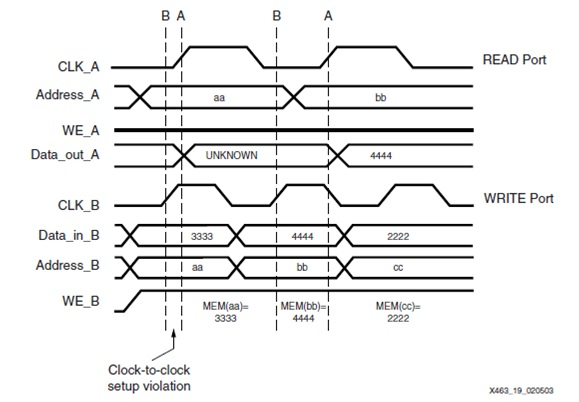
\includegraphics[width=\textwidth]{img/blockRam/conflittiTemp.jpg}
\caption{Conflitti per temporizzazioni d'accesso a Block Ram Dual-Port}
\label{fig:conflittiTemp}
\end{figure} 

Nel primo caso, la porta B inizia la scrittura in memoria all'indirizzo aa del dato 3333 e poco dopo, prima che la scrittura abbia terminato, arriva il fronte del CLK\_A che fa iniziare la lettura allo stesso indirizzo aa violando il tempo di setup necessario per scrivere il dato in memoria. Nel secondo caso invece si ha la scrittura da parte della porta B all'indirizzo bb del dato 4444 e in questo caso CLK\_A rispetta le temporizzazioni di scrittura e la porta A legge il dato correttamente scritto in memoria.\\

	\item Scrittura e Lettura contemporanea sulla stessa zona di memoria in funzione del WRITE\_MODE impostato (Fig.\ref{fig:conflittiScritture}).\\
Nei casi di scrittura su una porta e lettura sull'altra, se si utilizza WRITE\_MODE= NO\_CHANGE o WRITE\_FIRST, la scrittura su una porta invalida automaticamente il contenuto del registro di output (in lettura) dell'altra porta. Per tale motivo \`e consigliabile la modalit \`a di scrittura READ\_FIRST per evitare il problema dell'invalidazione del dato della porta in lettura.\\

\begin{figure}[!h]
\centering
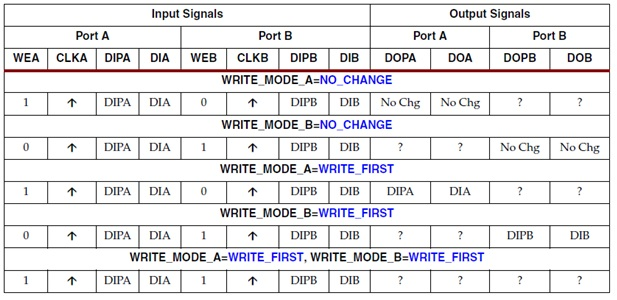
\includegraphics[scale=0.8]{img/blockRam/conflittiScritture.jpg}
\caption{Conflitti in lettura e scrittura simultanea come side-effect della WRITE\_MODE selezionata.}
\label{fig:conflittiScritture}
\end{figure}

\end{enumerate}

Per semplicit\`a implementativa la Block Ram non implementa un sistema di arbitraggio per gestire tali conflitti che sono lasciati a cura del progettista e comunque in caso di conflitto dovuto a scritture contemporanee non si verificano danni fisici al dispositivo di memoria. 

\section{Utilizzo della Block Ram in un progetto su FPGA}
La Block Ram pu\`o essere utilizzata in un progetto su FPGA per implementare una serie di funzionalit\`a che coinvolgano la memorizzazione di dati. I principali possibili utilizzi sono i seguenti:
\begin{enumerate}
\item RAM utilizzata da un microprocessore integrato sull'FPGA per memorizzare dati accessibili in lettura e scrittura.
\item ROM realizzata attraverso l'inizializzazione del suo contenuto all'avvio del sistema e accessibile in sola lettura.
\item Memorie FIFO.
\item etc.
\end{enumerate}

Tipicamente per utilizzare la Block Ram all'interno di un progetto si procede come segue:\\
\begin{enumerate}
\item Si crea un componente che utilizza la Block Ram configurandolo in base alle specifiche di progetto, settando il numero di porte volute,
l'ampiezza dei dati da trasferire, la dimensione della ram voluta,
etc.\\
Tale operazione pu\`o essere fatta in due modi:
\begin{enumerate}
\item Ricorrendo ad una serie di template presenti tra i Language Templates Ram di ISE appartenenti alla libreria UNISIM.
\item Configurazione ad hoc tramite Xilinx Core Generator che tramite un wizard consente di personalizzare il componente Ram di cui si ottiene infine il codice VHDL o Verilog.
\end{enumerate}
\item Si integra il componente all'interno del progetto dichiarandolo
nell'Architecture del componente finale e creandone un
istanza utilizzata internamente al progetto tramite degli appositi segnali interni.\\
Per utilizzare tali componenti implementati da Xilinx \`e necessario dichiare all'interno del progetto l'utilizzo della seguente libreria:

\lstset{language=VHDL, caption=Libreria dei Components Xilinx predefiniti, label=DescriptiveLabel, breaklines=true, basicstyle=\footnotesize\ttfamily, showspaces=false, showtabs=false, showstringspaces=false,  tabsize=3}
\begin{lstlisting}
library UNISIM;
use UNISIM.VComponents.all;
\end{lstlisting}

\item Si utilizza il componente che rappresenta la Block Ram comandando
i segnali di input e gestendo opportunamente i valori in
output.
\end{enumerate}


\clearpage{\pagestyle{empty}\cleardoublepage}
\chapter{Progetto d'esempio: BlockRam\_cmp}

%\section{Progetto d'esempio: BlockRam\_cmp}

Al fine di testare il funzionamento della Block Ram e approfondire le problematiche che vi sarebbero state nel progettare una cache reale che si interfacci con una Ram esterna il cui tempo di accesso non \`e nullo, abbiamo realizzato un componente Ram ad hoc: \texttt{BlockRam\_cmp}. Tale componente rappresenta una memoria Ram sincrona (il cui funzionamento \`e scandito dal clock in ingressso) realizzato con lo scopo di interfacciarsi con il nostro componente cache scambiando con questo linee di memoria di dimensione configurabile tramite un apposito parametro.\\
In questo caso, differentemente dall'implementazione realizzata nel \texttt{Ram\_cmp} del progetto, la memorizzazione dei dati non � pi� gestita tramite un array di linee di memoria a cui si accede istantaneamente, ma tramite un componente interno \texttt{RAMB16\_S9} capace di trasferire singoli byte ad ogni ciclo di lettura o scrittura.

\section{Specifiche del progetto}
\begin{itemize}
\item \texttt{BlockRam\_cmp} \`e il componente che si occupa di gestire le richieste di lettura e scrittura di linee in memoria Block Ram. 
\item La dimensione in byte della linea di memoria � configurabile tramite l'apposita costante \texttt{nbyte\_line} della libreria.
\item Utilizzo di 1 componente Block Ram di dimensione 18 Kbits con organizzazione interna 2Kx9, ovvero ram-depth pari a 2048 ed ampiezza del dato trasferito di 9 bit (di cui 8 di dato e 1 di parit\`a trascurato nel progetto).
\item Il componente \texttt{BlockRam\_cmp} ha lo scopo di interfacciarsi internamente con la Block Ram per gestire una sequenza di \texttt{nbyte\_line} trasferimenti da o verso la Block Ram al fine di leggere o scrivere in memoria un'intera linea di memoria. 
\end{itemize}

\section{Implementazione}
Per comodit\`a abbiamo ipotizzato che il componente \texttt{BlockRam\_cmp} si interfacci alla cache sempre tramite un bus dati dell'ampiezza della linea di memoria da trasferire. Tale ipotesi semplificativa porta ad una potenziale complessit\`a del cablaggio del bus dati, ma \`e tuttavia lecita dal momento che i trasferimenti tra cache e ram coinvolgono sempre linee di memoria. Ci\`o detto, il nuovo componente prevede l'utilizzo al suo interno del componente Block Ram \texttt{RAMB16\_S9} capace di leggere e scrivere dati da 8 bit. La scelta di tale organizzazione della Block Ram deriva dall'ipotesi che le linee di memoria sono sempre di dimensione multipla di 8 bit (1 Byte) e quindi il componente \texttt{BlockRam\_cmp} ad ogni operazione di lettura o scrittura di una linea dove provvedere ad un ciclo di trasferimento dei singoli Byte costitutivi la linea a partire dall'indirizzo specificato in ingresso sul bus degli indirizzi che ad ogni accesso dovr\`a essere incrementato opportunamente.\\ In alternativa si sarebbero potuti trasferire dati anche maggiori (fino a 32 bit) ma l'effetto sarebbe stato quello di avere un vincolo ulteriore sulla dimensione della linea che sarebbe stata multiplo di un maggiore numero di byte (4 byte nel caso di trasferimenti a 32 bit in Block Ram).\\

\lstset{language=VHDL, caption=Il codice seguente mostra l' inizializzazione fatta nel progetto d'esempio del contenuto interno della Block Ram tramite gli attributi INIT\_xx\, SRVAL\, INIT e le modalit\`a di scrittura WRITE\_MODE., label=DescriptiveLabel, breaklines=true, basicstyle=\footnotesize\ttfamily, showspaces=false, showtabs=false, showstringspaces=false,  tabsize=3}
\begin{lstlisting}
component RAMB16_S9 --DATA_WIDTH=8 RAM_DEPTH=2048

--configurazione attributi della Block Ram
generic (
	
	WRITE_MODE : string := "READ_FIRST" ; -- WRITE_FIRST(default)/ READ_FIRST/NO_CHANGE
	
	-- valore in output dopo inizializzazione
	INIT : bit_vector(35 downto 0) := X"000000000";
	
	-- valore letto in caso di asserimento del segnale SSR
	SRVAL : bit_vector(35 downto 0) := X"000000002";
	
	-- Inizializzazione del contenuto della Block Ram
	 INIT_00 : bit_vector := X"0000000000000000000000000000000000000000000000000F00FFFFFFFFFFFF";
    INIT_01 : bit_vector := X"100000000000000000000000000000000000000000000000000000000000000F";
	 ...
    INIT_3E : bit_vector := X"0000000000000000000000000000000000000000000000000000000000000000";
    INIT_3F : bit_vector := X"000000000000000000000000000000000000000000000000000000000000000F"
	);
	
	port(
		DI: in std_logic_vector (DATA_WIDTH-1 downto 0);
		DIP: in std_logic_vector (0 downto 0);
		DO: out std_logic_vector (DATA_WIDTH-1 downto 0);
		DOP: out std_logic_vector (0 downto 0);
		ADDR: in std_logic_vector (ADDR_BIT-1 downto 0);
		WE: in std_logic;
		EN: in std_logic;
		CLK: in std_logic;
		SSR: in std_logic
	);
end component;

\end{lstlisting}


La Fig. \ref{fig:br_cmp} mostra una schematizzazione dei process utilizzati per gestire le funzionalit\`a sopra descritte.\\

\begin{figure}[!h]
\centering
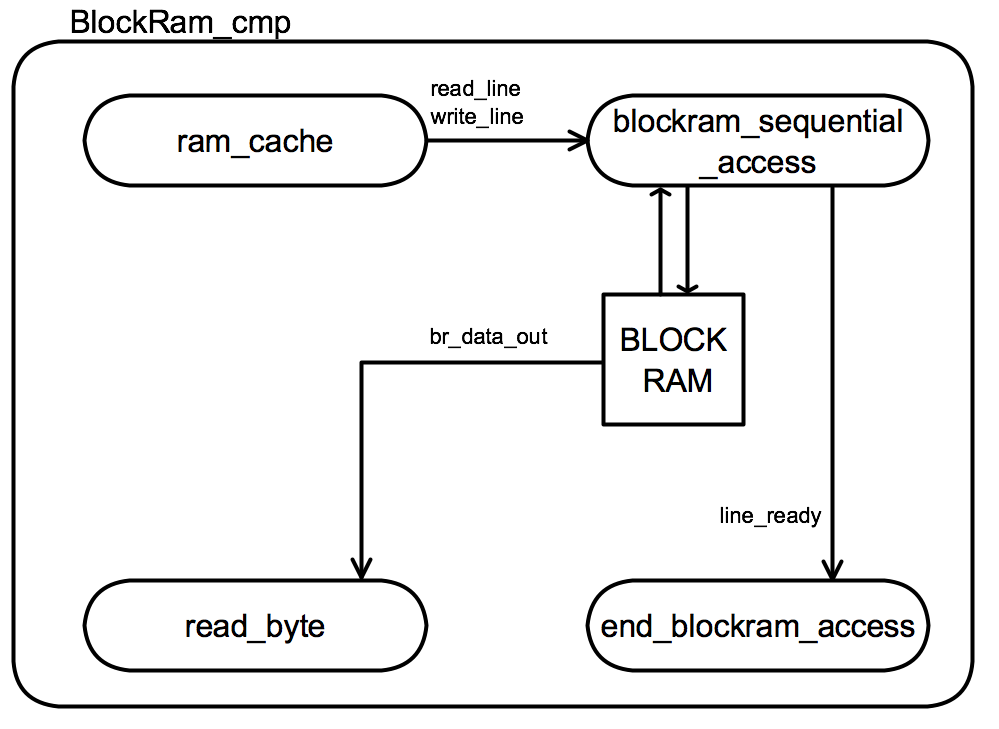
\includegraphics[width=\textwidth]{img/blockRam/blockram_cmp.png}
\caption{Schematizzazione dei processi che gestiscono la Block Ram}
\label{fig:br_cmp}
\end{figure}

\subsection{ram\_cache}
Il process \texttt{ram\_cache} � il processo principale che gestisce le richieste di trasferimento di linee di memoria provenienti dalla cache. Tale processo sulla base dei segnali di comando ricevuti (\texttt{en}, \texttt{memrd} e \texttt{memwr}) asserisce i segnali interni di sincronizzazione, abilitando le seguenti operazioni:
\begin{enumerate}
\item \texttt{write\_line}: la scrittura di una linea in Block Ram deve provvedere al trasferimento byte per byte della linea in ingresso su \texttt{bdata\_in} sulla Block Ram tramite una serie di \texttt{nbyte\_line} scritture consecutive che avvengono sul fronte positivo del clock \texttt{clk} in ingresso alla Block Ram.
\item \texttt{read\_line}: la lettura di una linea da Block Ram deve prevedere un buffer (una variabile VHDL \texttt{line} di tipo \texttt{mem\_line}) che viene riempito man mano attraverso \texttt{nbyte\_line} letture di byte dalla Block Ram. Al termine la linea letta deve essere restituita in uscita alla cache su \texttt{bdata\_out} (bus dati di output).
\end{enumerate}

\subsection{blockram\_sequential\_access}
Il process \texttt{blockram\_sequential\_access} si occupa di gestire tramite un contatore interno gli accessi sequenziali alla Block Ram, scanditi dal clock \texttt{clk}. Tali accessi in sequenza saranno in lettura qualora \texttt{read\_line} \`e asserito, in scrittura se \`e asserito il segnale \texttt{write\_line}. \\Per tale motivo questo process ha la responsabilit\`a di incrementare l'indirizzo di memoria dopo ogni accesso e comandare tramite opportuni segnali interni le operazioni di lettura e scrittura di singoli byte sulla Block Ram RAMB16\_S9.\\

Tali segnali interni sono mostrati nel port map del componente RAMB16\_S9:

\lstset{language=VHDL, caption=Port Map del componente RAMB16\_S9 - collegamento ai segnali interni utilizzati per interfacciarsi alla Block Ram., label=DescriptiveLabel, breaklines=true, basicstyle=\footnotesize\ttfamily, showspaces=false, showtabs=false, showstringspaces=false,  tabsize=3}
\begin{lstlisting}
RAMB16_S9_inst : RAMB16_S9
	port map
	(
		DI => br_data_in (DATA_WIDTH-1 downto 0),
		DIP => br_parity_in,
		DO => br_data_out (DATA_WIDTH-1 downto 0),
		DOP => br_parity_out,
		ADDR => br_addr (ADDR_BIT-1 downto 0),
		WE => br_we,
		EN => br_en,
		CLK => clk,
		SSR => br_ssr
	);
\end{lstlisting}


Mentre in scrittura il processo \texttt{blockram\_sequential\_access} gestisce correttamente la sequenza di scritture in quanto il contatore degli accessi aggiorna a ogni clock l'indirizzo in scrittura e il byte della linea da scrivere a tale indirizzo, in caso di lettura ci\`o non \`e altrettanto immediato.\\
Il motivo \`e che per leggere un byte a ogni ciclo di lettura si fornisce alla Block Ram l'indirizzo a cui leggere il dato ed il segnale \texttt{en} per abilitare la lettura, ma tale dato non \`e immediatamente disponibile sul bus dati in uscita dalla Block Ram (\texttt{br\_data\_out}) in quanto bisogna attendere un tempo d'accesso in lettura per avere il dato richiesto.\\

Per risolvere tale problema, dal momento che la Block Ram non dispone di un segnale di ready col quale avvisare che il byte letto \`e pronto e non potendo utilizzare un processo asincrono che si attiva con una commutazione del bus dati di output della Block Ram a causa di possibili letture di dati uguali (che non attiverebbero il processo), abbiamo determinato il tempo necessario per completare la lettura di un byte. Abbiamo verificato, tramite prove pratiche (non avendo trovato indicazioni temporali sui tempi di accesso alla Block Ram nel materiale consultato della User Guide di Xilinx), che il dato letto viene reso disponibile in uscita alla Block Ram con l'arrivo del secondo clock. In base a tale tempistica ogni qualvolta si effettua la lettura di un byte il contatore viene incrementato per procedere nella sequenza di letture dopo 2 clock quando il dato sar\`a sicuramente presente per essere letto. In questo modo si leggono correttamente i byte richiesti che vengono caricati nella linea di memoria che verr\`a portata in uscita al termine della sequenza di letture.

\subsection{end\_blockram\_access}
Il process \texttt{end\_blockram\_access} viene risvegliato ogni qual volta si attiva il segnale \texttt{line\_ready} col quale il process \texttt{blockram\_sequential\_access} avvisa che il trasferimento della linea \`e stato completato. La responsabilit\`a di tale process \`e quindi di attivare il segnale di \texttt{ready} e in caso di lettura fornire la linea letta all'esterno portandola in uscita sul bus dati \texttt{bdata\_out}. Lo stesso, a fini didattici, accade anche in caso di scrittura al fine di testare il funzionamento della Block Ram con le diverse WRITE\_MODE.\\

\section{Testbench}
Per verificare il funzionamento del componente abbiamo realizzato un semplice testbench nel quale si scrive all'indirizzo 0000h della Block Ram la linea di dimensione configurabile tramite parametro (8 byte nel nostro esempio) passata in ingresso sul bus \texttt{bdata\_in}.
Successivamente si effettua una lettura allo stesso indirizzo per verificare l'effettiva scrittura del dato in memoria.\\
Al fine di verificare le diverse modalit\`a di funzionamento in scrittura della Block Ram descritte in precedenza, abbiamo provato lo stesso test sul componente configurando le tre differenti politiche di scrittura possibili.\\
\begin{figure}[!h]
\centering
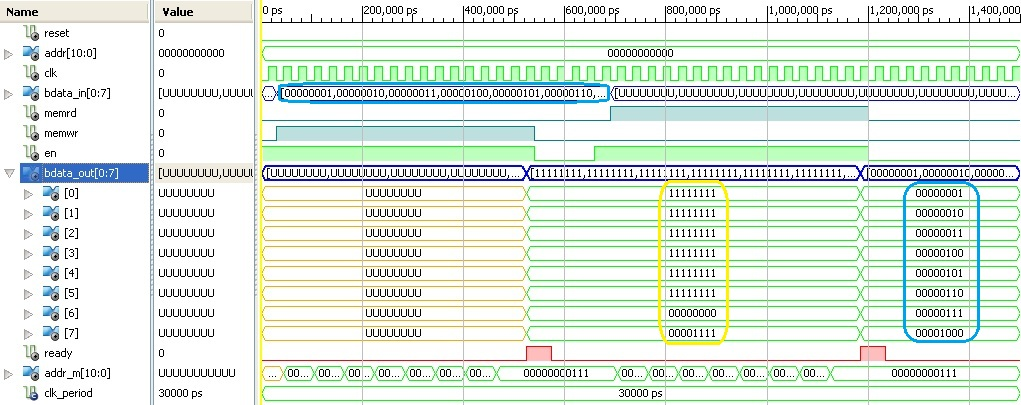
\includegraphics[width=\textwidth]{img/blockRam/test_read_first.jpg}
\caption{Simulazione con WRITE\_MODE = READ\_FIRST}
\label{fig:sim-rf}
\end{figure}
Il primo caso \`e quello di scrittura in modalit\`a READ\_FIRST in Fig.\ref{fig:sim-rf}. Ovvero in questo caso l'operazione di scrittura di una linea sulla Block Ram, oltre all'attivazione del segnale di ready, comporta in uscita sul bus dati \texttt{bdata\_out} una linea di memoria il cui contenuto sono gli 8 byte (nel cerchio in giallo) presenti sulla Block Ram che verranno sovrascritti.\\
Tale modalit\`a consente quindi di verificare anche la corretta inizializzazione del contenuto della Block Ram fatta all'interno della sezione generic(...).

Il secondo caso (in Fig.\ref{fig:sim-wf}) \`e caratterizzato dalla politica di scrittura di default, ovvero la WRITE\_FIRST. Tale politica come mostra la simulazione, consente durante un ciclo di scrittura di avere contemporaneamente la scrittura del dato in ingresso sia in memoria all'indirizzo specificato sia sui latch di output.
\begin{figure}[!h]
\centering
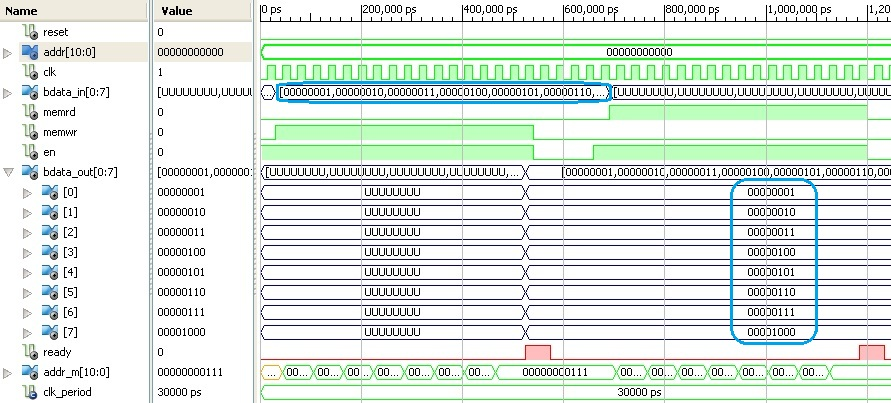
\includegraphics[width=\textwidth]{img/blockRam/test_write_first.jpg}
\caption{Simulazione con WRITE\_MODE = WRITE\_FIRST}
\label{fig:sim-wf}
\end{figure}

Infine in Fig.\ref{fig:sim-nc} abbiamo il caso di scrittura in modalit\`a NO\_CHANGE che non comporta alcun cambiamento del contenuto dei latch in output in caso di scrittura che rimane al valore nullo di default dal momento che non erano state fatte letture in precedenza.
\begin{figure}[!h]
\centering
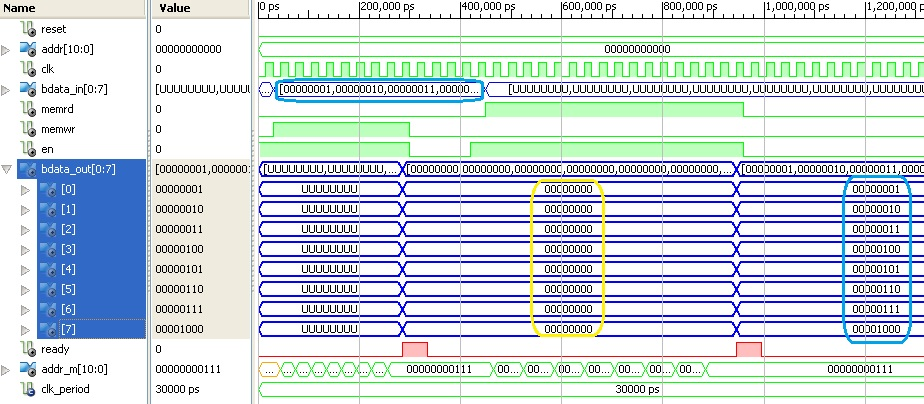
\includegraphics[width=\textwidth]{img/blockRam/test_no_change.jpg}
\caption{Simulazione con WRITE\_MODE = NO\_CHANGE}
\label{fig:sim-nc}
\end{figure}

\section{Considerazioni sul progetto d'esempio}

Il componente BlockRam\_cmp rappresenta una memoria RAM a tutti gli effetti che prevede dei tempi d'accesso non nulli sia in scrittura che in lettura. Ci\`o comporta la necessit\`a di tenere in conto i tempi d'accesso alla memoria al fine di segnalare opportunamente (segnale di \texttt{ready}) alla cache quando possa leggere il dato richiesto (nel caso del nostro progetto che prevede il ready in ingresso alla cache per la sincronizzazione). Al termine dell'analisi del funzionamento della Block RAM e del componente realizzato abbiamo provato a integrarlo con la nostra \texttt{Cache\_cmp} utilizzando i testbench precedenti, sostituendo il componente \texttt{Ram\_cmp} con il  nuovo. L'integrazione ha avuto esito positivo.\\

Nell'ottica di una possibile integrazione con il processore DLX, si dovrebbero gestire le temporizzazioni d'accesso alla Block RAM, inserendo gli stati di wait e il segnale di \texttt{ready} in ingresso in modo da essere informato del completamento di un ciclo d'accesso alla memoria.\\
L'utilizzo del \texttt{ready} significherebbe dover introdurre esternamente un contatore che, a ogni accesso in memoria sulla base dei tempi d'accesso e dei ritardi presenti sulla rete, conti quanti stati di wait sono necessari al fine di completare l'accesso e generi opportunamente il ready da inviare al processore. Dal punto di vista dell'implementazione interna del DLX ci\`o comporterebbe la necessit\`a di stallare la pipeline qualora il ready non sia asserito.
